
\chapter{Stacking Methodology}
Given the signal from a single filament is well below the level of noise in a given $y$ map, in order to effectively detect the signal for the filaments, we need to add many individual sources together. Because the noise, and the signal in the CMB is presumed to be gaussian, the expectation is that correlated signals would add, and uncorrelated signals would be driven to zero. This means that by adding together thousands of signals lower than the signal-to-noise ratio of a given $y$ map, it should show the filaments as a correlated signal, along with their corresponding galactic halos.

Initially outlined in \cite{2016MNRAS.457.2391C}, the stacking algorithm involves creating a list of galaxy pairs, which we would expect to see a filament between, and then using those pairs, forming a normalised two-dimensional image, with the galaxies of the pair being placed on two points in the image, and stacking them until the signal to noise is sufficient to be measurable.

The intial problem faced involves generating the galaxy pairs from the Dark Energy Survey redMaGiC Catalogue. The Year 1 Catalogue consists of 0.65 million red-sequence galaxies in the redshift range $0.15 < z < 0.9 $. The algorithm used by the Dark Energy Survey to select these red-sequence galaxies provides redshift estimates of very high quality and very low bias ($\lesssim 0.5$ percent). They also have very low scatter, and a very low rate of catastrophic outliers. The algorithm yields superior photo-z performance than the colour-cut methodology used to define the Sloan Digital Sky Survey CMASS catalogue \citep{2016MNRAS.461.1431R}. 

The DES catalogue has a larger footprint than the SPTpol viewing footprint, so we first have to exclude any galaxies that lie outside of the SPTpol area. The SPTpol observing area consists of a 500 square degree patch of sky, extending from an Right Acension (RA) of 22h to 2h, and a Declination (Dec) of -52 degrees to -67 degrees. Excluding any galaxies outside this region yields approximately 100000 galaxies, less than a sixth of the original catalogue. 

\begin{figure}[h!]
\centering 
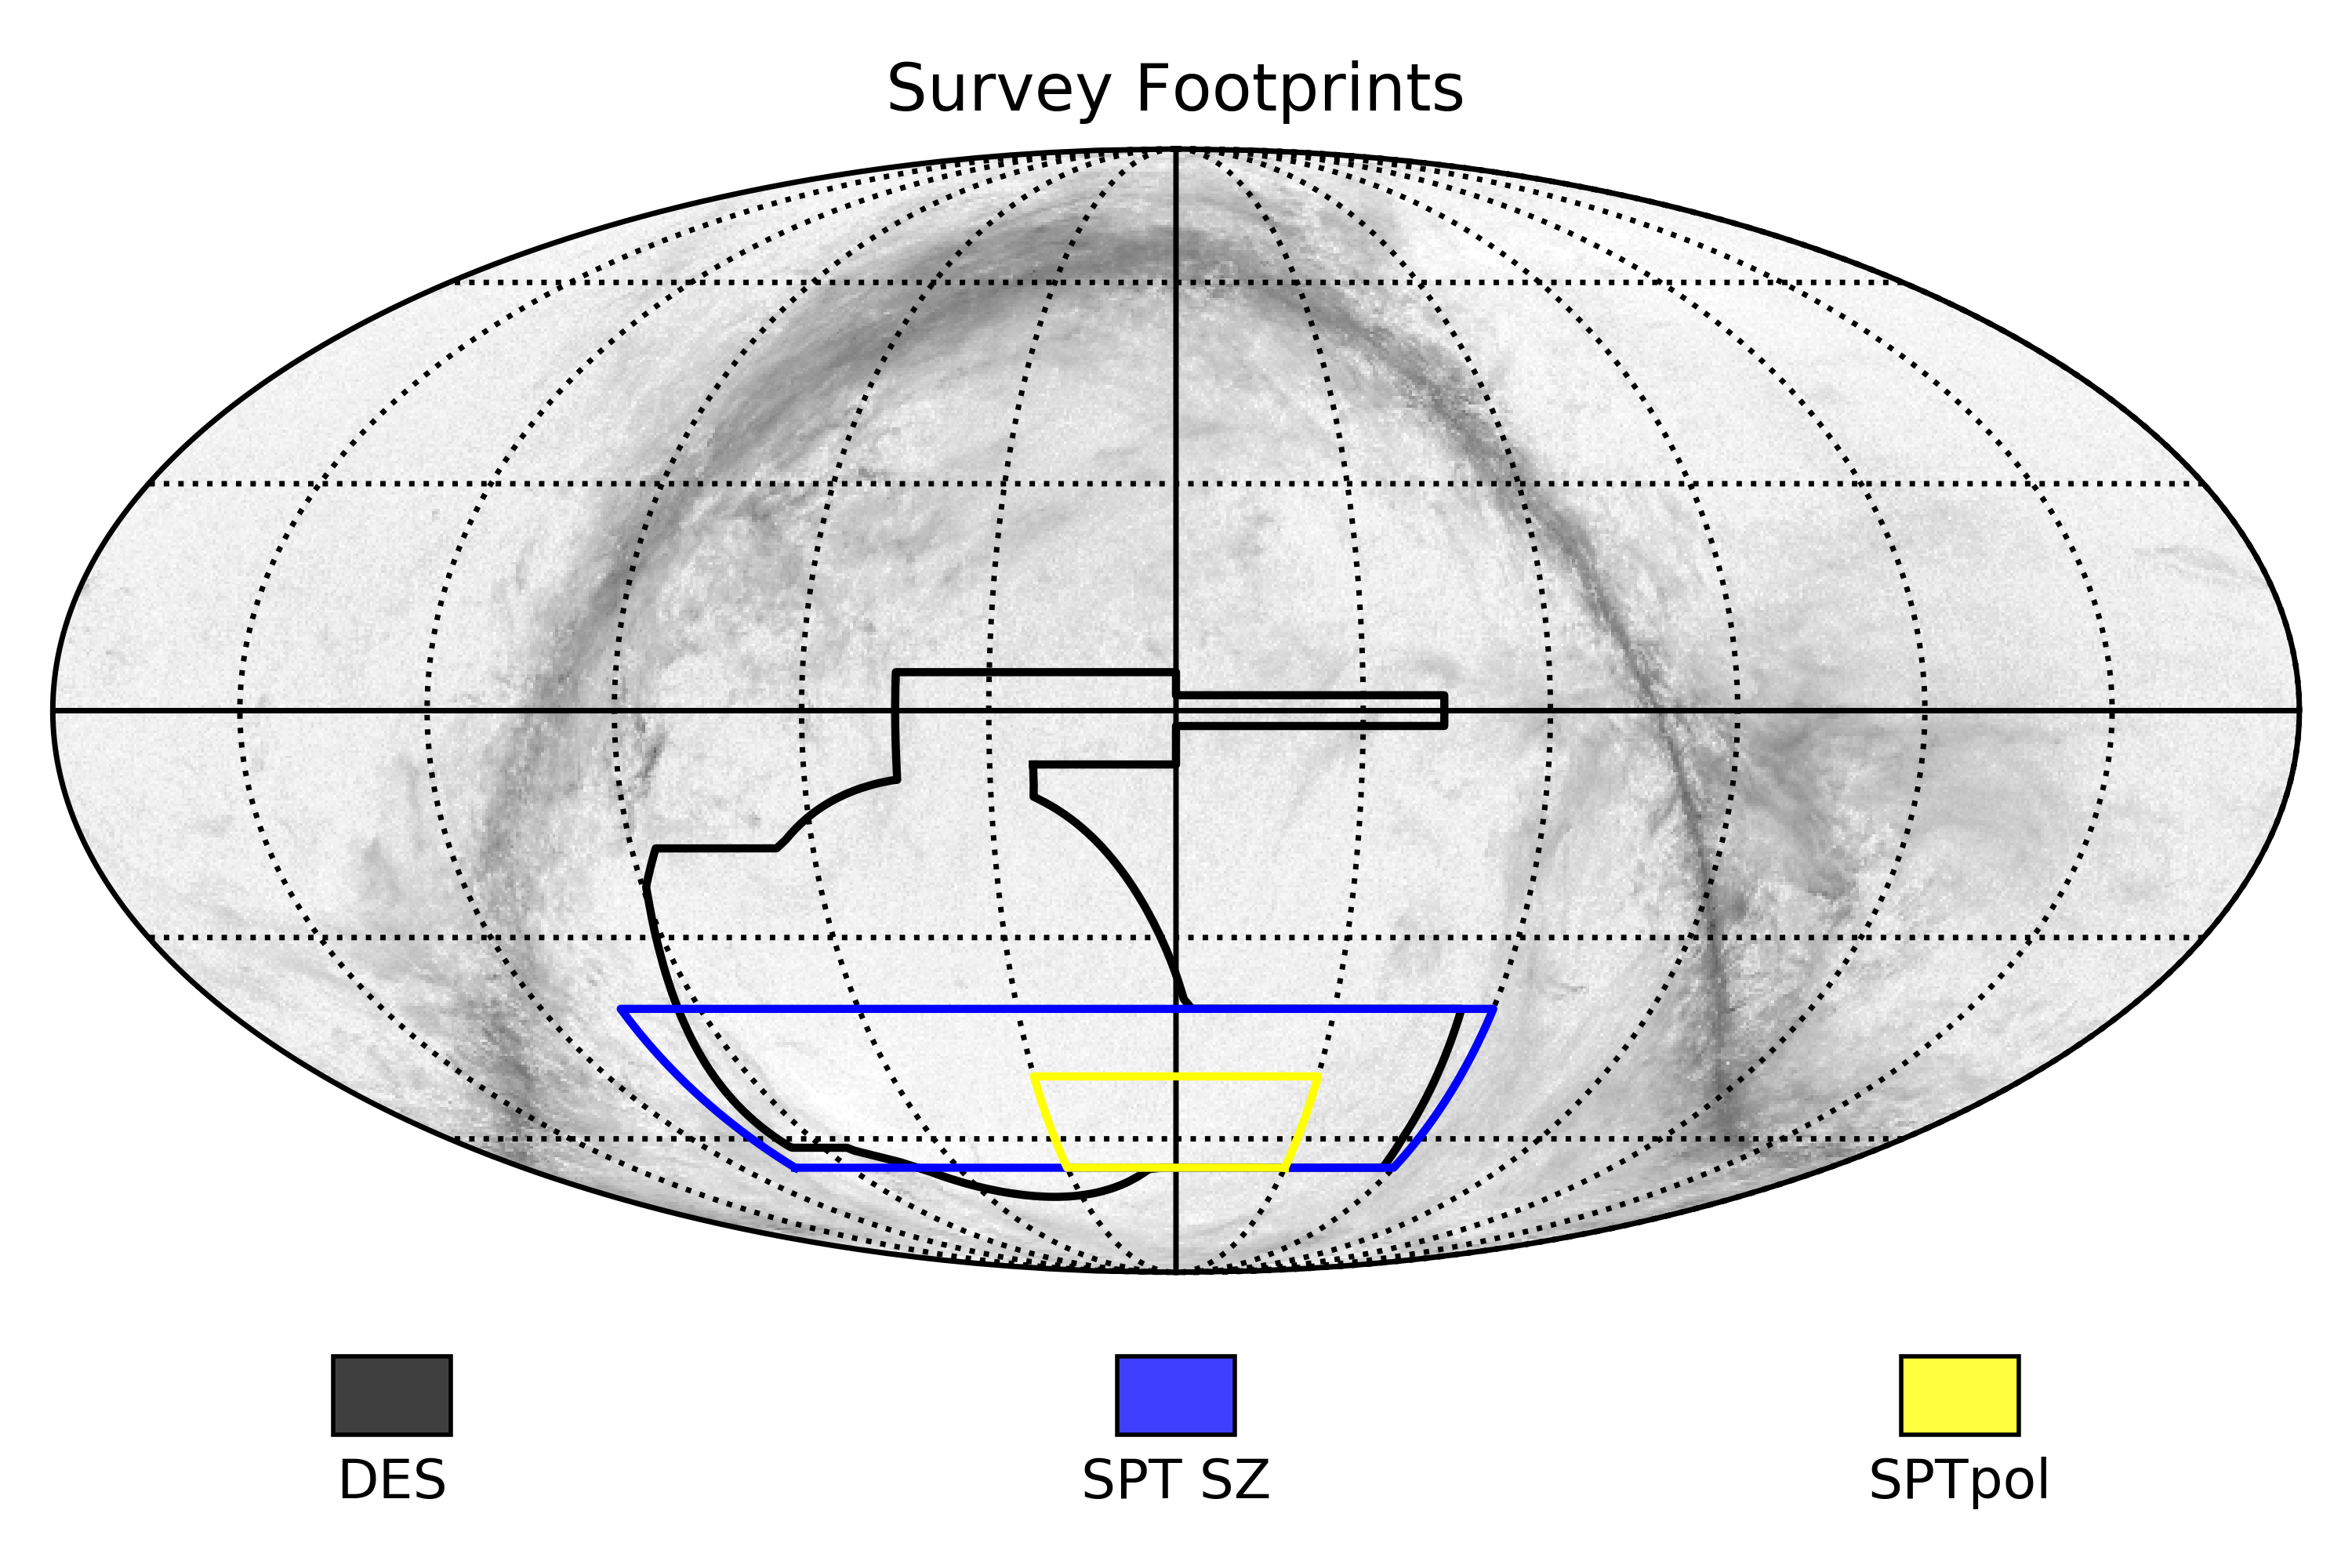
\includegraphics[scale=0.7]{/home/mitchell/Documents/masters/masters/thesis/Ver_2/figures/Survey_Outlines.png}
\caption{Outlines of SPTpol, SPT-SZ, and DES surveys}
\label{fig:surveys}
\end{figure}



Pairs were generated by making use of kD-trees. A generalisation of a binary tree, the kD tree is one where every leaf node is representative of a $k$ dimensional point. Each non-leaf node is one that 'splits' the space into two parts, whereby points to the left of this hyperplane are represented by the left sub-tree, and to the right are represented by the right sub-tree. When we apply this to our galaxy catalogue, we first locate them in 3 dimensional space, by converting their RA, Dec, and redshift into a comoving 3D coordinate. They are then placed in a kD tree, and any pair which has a radial comoving separation of less that $10 h^{-1} $ Mpc, and transverse comoving separation range of $6 - 14 h^{-1} $ Mpc is considered to have a filament \citep{2016MNRAS.457.2391C}.


\begin{figure}[h!]
\centering
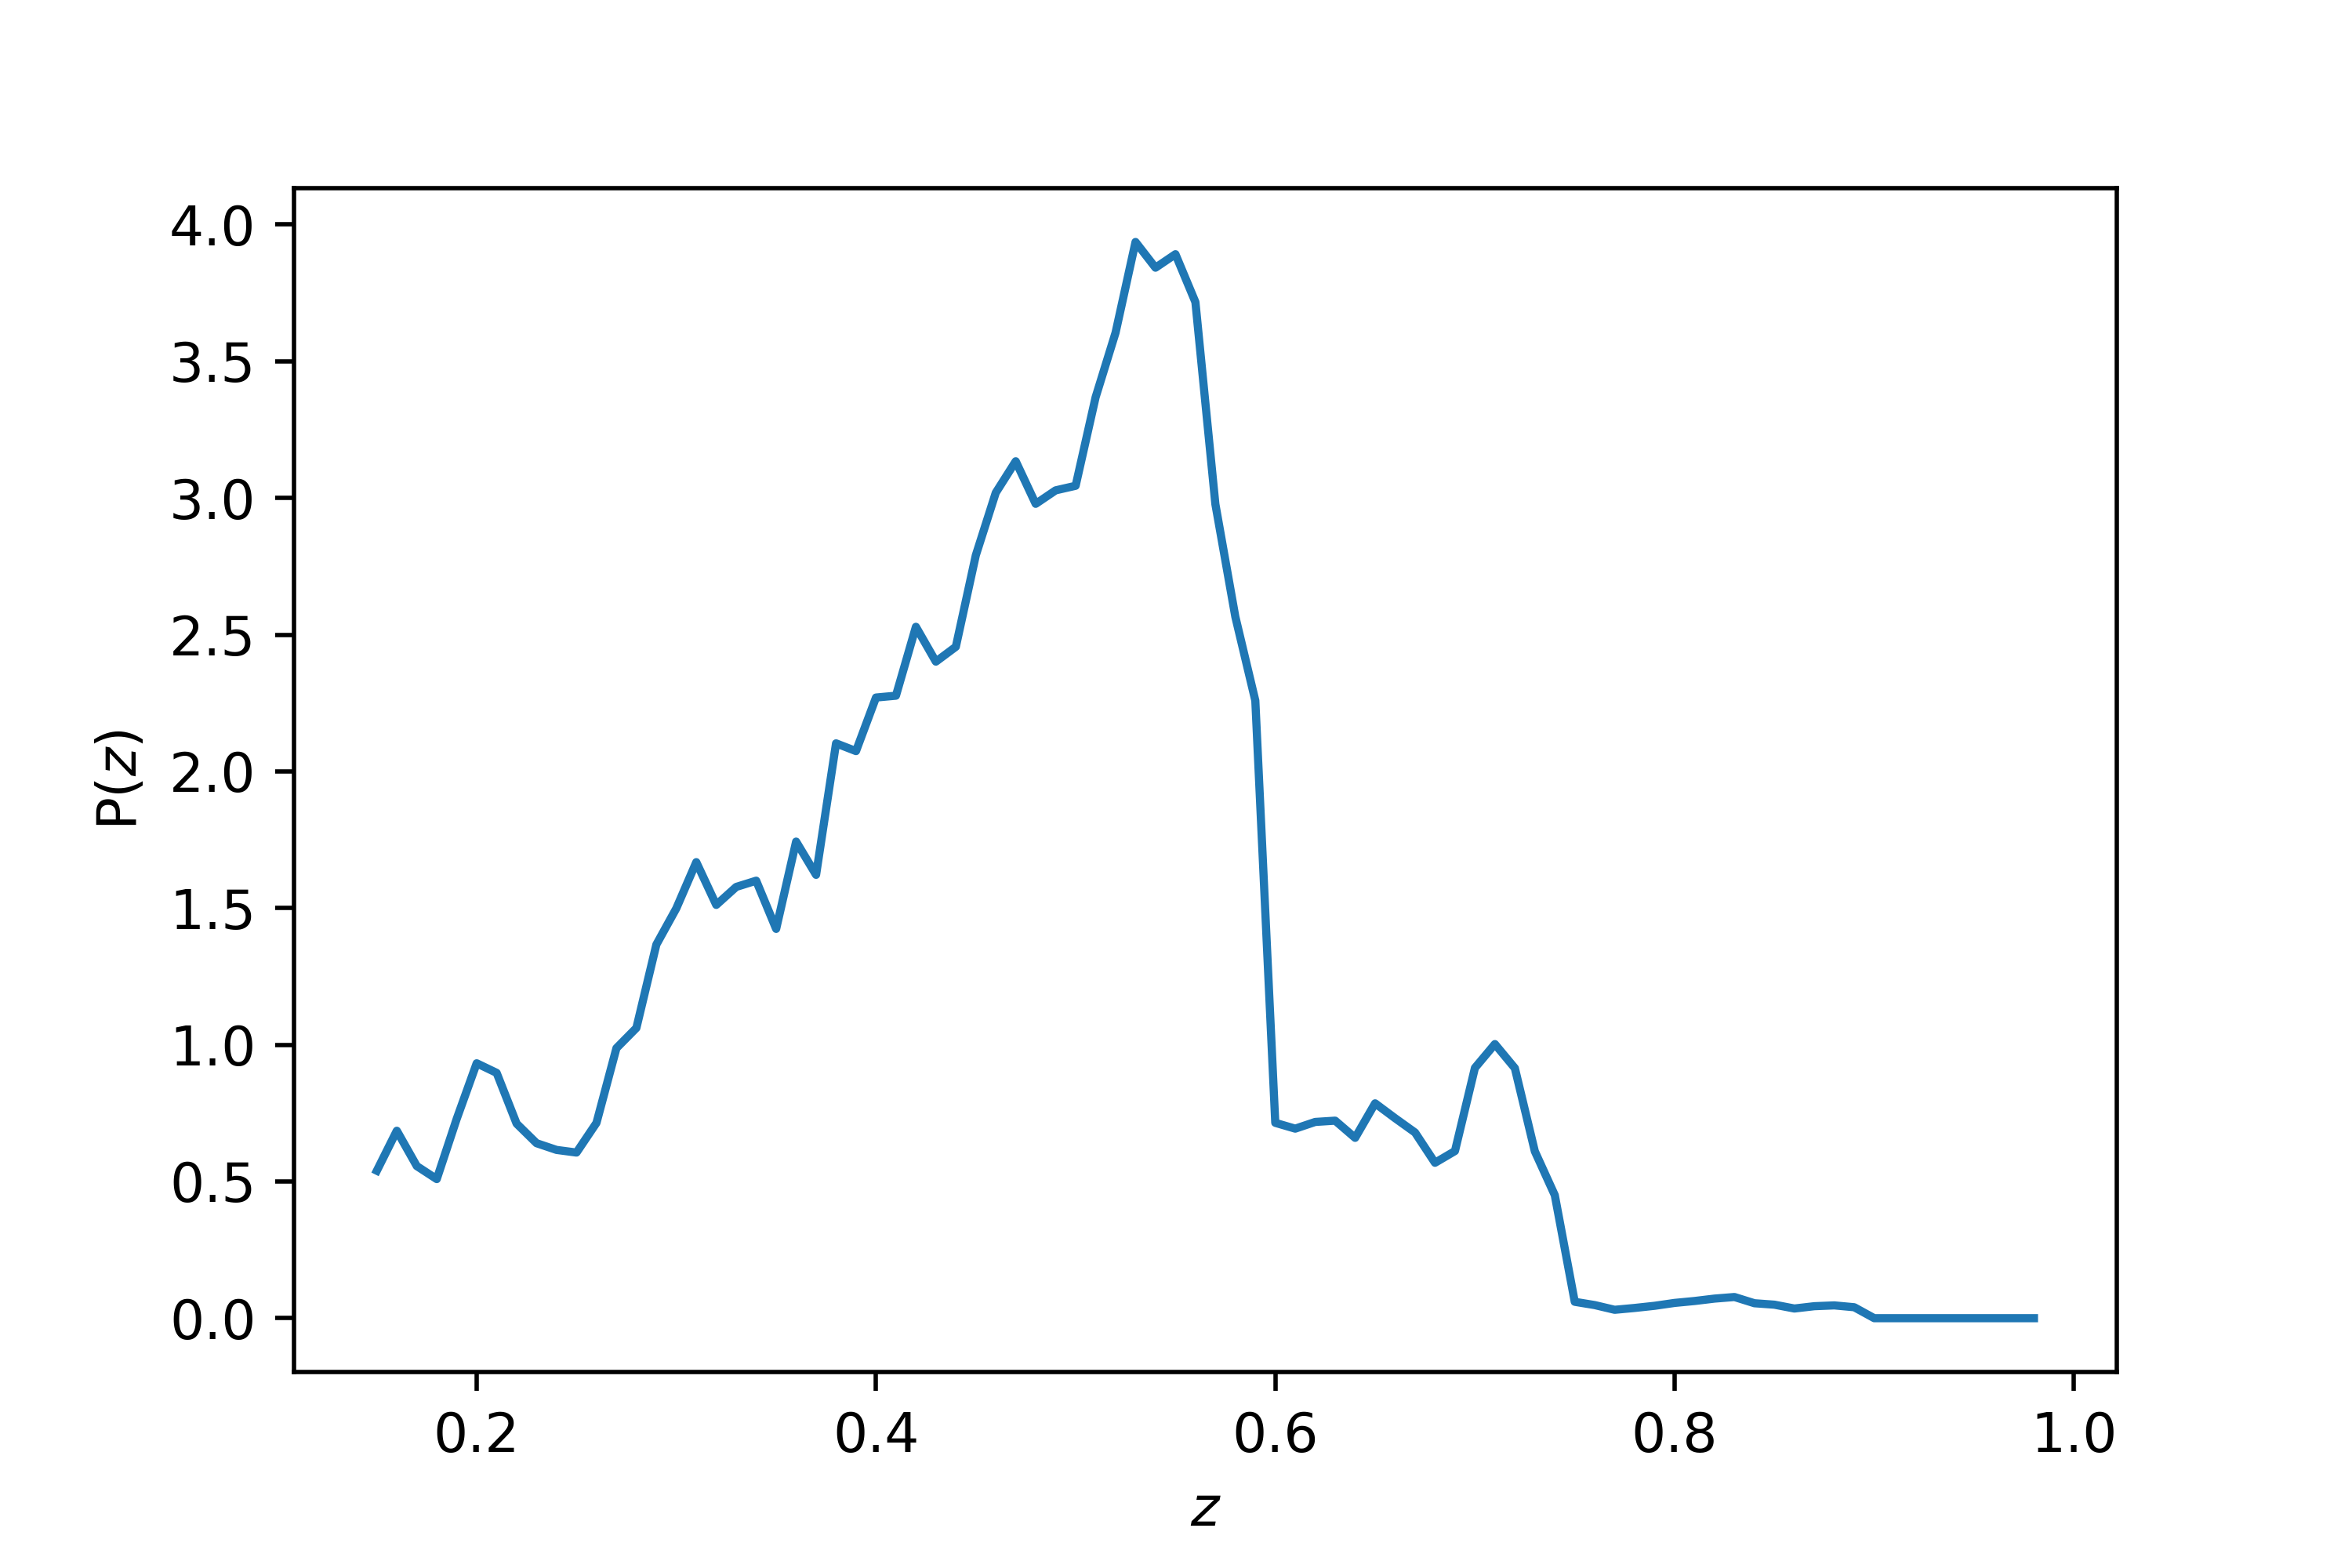
\includegraphics[scale=0.7]{/home/mitchell/Documents/masters/masters/thesis/Ver_2/figures/Redshift_Distribution.png}
\caption{Redshift Distribution of Galaxy Pairs}
\label{fig:pairs_dist}
\end{figure}

Figure \ref{fig:pairs_dist} shows the overall distribution of galaxy pairs as a function of redshift. It shows that the mean redshift for the pairs is $z=0.468$, with a minumum redshift of $z= 0.150$, and a maximum redshift of $z= 0.899$. There is a rather drastic drop in the galaxy population after redshift $z \sim 0.58$. This is due to there being fewer galaxies in the higher redshift bins in the DES Year 1 Catalgogue.  


Functionally, this algorithm follows some elementary primary operations:
\begin{enumerate}[label=(\Roman*)]
\item A pair is located in the CMB \label{step:1}
\item A slice is taken around the pair \label{step:2}
\item The slice is then rotated, so that the pair is aligned along the same axis \label{step:3}
\item The slice is then rescaled, so that each element of the pair is situated at the same point in pixel space \label{step:4}
\item These slices are then mirrored, in both the $x$ and $y$ axes separately and then together, and the average is taken over all four mirror images \label{step:5}
\item These averages are then co-added, and the average is taken over the number of pairs added together \label{step:6}
\end{enumerate}
%\FloatBarrier

%\begin{figure}[h!]
%\centering 
%\includegraphics[scale=0.8]{/home/mitchell/Documents/masters/masters/data/server/run_42/steps/1_firstcut.png}
%\caption{Initial Slice of CMB}
%\label{fig:first_cut}
%\end{figure}

Steps \ref{step:5} and \ref{step:6} are done by applying an affine transformation to the array of values, because we are seeking to preserve the functional position of all points, straight lines, and ratios in the array, as close to the original as possible. 

%\begin{figure}[h!]
%\centering 
%\includegraphics[scale=0.8]{/home/mitchell/Documents/masters/masters/data/server/run_42/steps/1_rotated.png}
%\caption{Rotated Cut-Out}
%\label{fig:rotated}
%\end{figure}


%\begin{figure}[h!]
%\centering 
%\includegraphics[scale=0.8]{/home/mitchell/Documents/masters/masters/data/server/run_42/steps/1_rescaled.png}
%\caption{Rescaled Cut-Out}
%\label{fig:rescaled}
%\end{figure}

 
%\begin{figure}[h!]
%\centering 
%\includegraphics[scale=0.8]{/home/mitchell/Documents/masters/masters/data/server/run_42/steps/1_secondcut.png}
%\caption{Second Cut-Out}
%\label{fig:second_cut}
%\end{figure}

We perform operations \ref{step:4} and \ref{step:5} because we make the assumption that the dark matter halos that host the LRGs we are considering are spherically symmetric. Mirroring the halos about two axes essentially allows us to stack multiple versions of each individual halo. Doing so reduces irregularities introduced by any halos that happen to be non-symmetric, whilst correlating their spherical structure. 

We tested this algorithm by creating dummy simulated datasets, where an artifical signal inserted in noise that is 3 to 4 orders of magnitude higher than it. 

\begin{figure}[h!]
\centering
\includegraphics[scale=0.4]{/home/mitchell/Documents/masters/masters/thesis/Ver_2/figures/simulated_stack.png}
\caption{Stacking Algorithm as applied to Dummy Data. (a) Slice is taken of a given pair, (b) Slice is rotated, aligning both elements of the pair with the $x$ axis, (c) Slice is rescaled. Axes scales have been left in to illustrate the relative scaling between (b) and (c), (d) Second slice is taken of the manipulated data}
\end{figure}

As can be clearly seen, there appears to be no signal in the individual slices of data, but when they are coadded and mirrored, the signals clearly appear as two bright halos. 

Some things to note about this method. First, there are some interesting artefacts along the lines of symmetry. Because both signal and noise are getting mirrored about two axes, any data that lies along one of these axes will get flipped, but will not move in place. This introduces some measure of artificial correlation, because any noise that lies along these axes will look like it is correlated with the un-mirrored data. This is clear in artefacts that lie along the vertical axis. 
%\begin{figure}
%\centering
%\includegraphics[scale=1]{/home/mitchell/Documents/masters/masters/data/server/run_42/steps/1_average.png}
%\caption{Average of Mirrored Arrays}
%\label{fig:average_cut}
%\end{figure}
Secondly, it is sensitive to the separation of the galaxy pair in pixel space. If a galaxy is relatively close together, the rescaling operation will stretch out the pair until they are located at the normalised positions chosen. This also has the effect of stretching out their halo as a whole. This means that pairs that are more separated in pixel space will be rescaled less, and so the halos will be more compact, and pairs that have a lower separation will be rescaled more, and so have a larger angular extent after rescaling. This essentially means that the halo sizes will not be evenly distributed, they will follow the distribution of the pair separations on the sky.  

\par Once we have the pairs co-added, we need to subtract the halo contribution. There are a number of possible ways to do this. We can analytically solve for the halo contribution in the map by using a model of the form 
\begin{equation}
y_h(p) = y_{L,i} + y_{R,j} 
\end{equation}
, where $p$ represents a given pixel, $L$ and $R$ indicate the left and right halos respectively, and $i$ is the $i$th radial bin from the centre of the left halo, and $j$ is the $j$th radial bin from the centre of the right halo. 

\par In order to avoid introducing bias from the potential filament, we exclude the central region of the stack, as shown in Figure \ref{fig:fit_mask}

\begin{figure}[h!]
\centering 
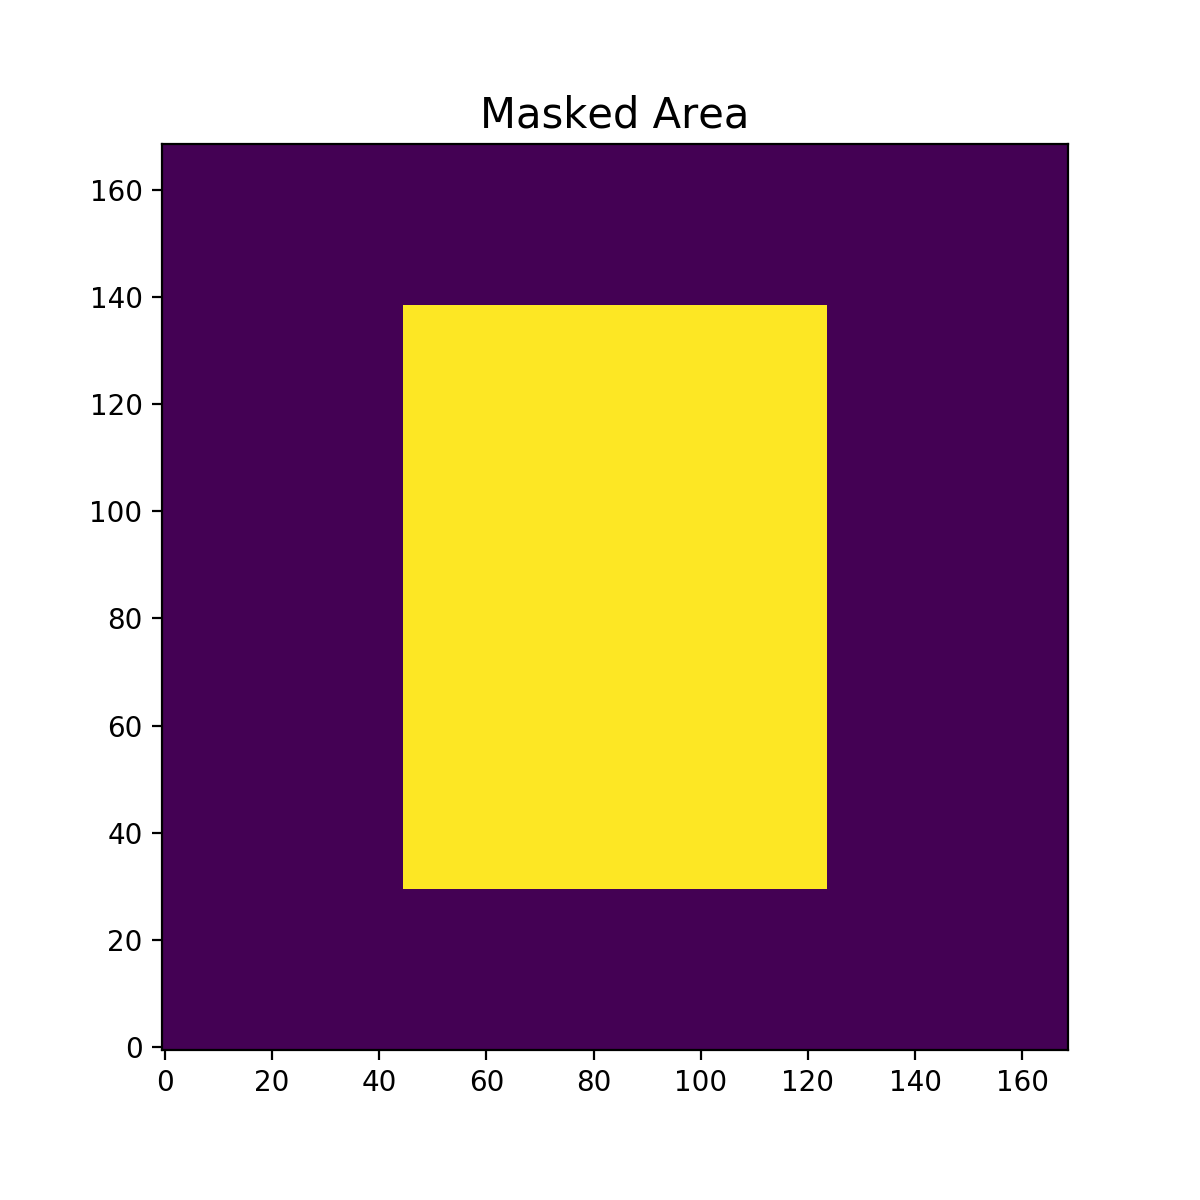
\includegraphics[scale=0.8]{/home/mitchell/Documents/masters/masters/thesis/Ver_2/figures/mask.png}
\caption{Area of galaxy pair stack masked from profile fit}
\label{fig:fit_mask}
\end{figure}



\section{Null Tests}

In order to test the validity of the detection, and make an estimate of its uncertainty, we perform several different types of Monte-Carlo based tests. 

\subsection{Random Rotation}
In the first test, we rotate pairs by a completely random angle. This test should produce a 
\subsection{Un-Physical Pairs}
The second test involves stacking the $y$ map against 'pseudo-pairs' of galaxies. These pairs satisfy the transverse separation condition, but do not satisfy the radial separation condition, having instead radial separations between $\SI{100}{\per\h}$ and $\SI{200}{\per\h}$ Mpc. Pairs with these conditions are not expected to have any filament connecting them, and the radial separation conditions have been calculated to take into account the errors assosciated with the photometric redshifts found in the Dark Energy Survey catalogue. 
\par In order to produce this pair set, we first calculate the total number of pairs that sit within approximately $\SI{0.5}{\degree}$ on the sky, and calculate their line of sight separations. We then determine the transverse separation of the pair, and apply the same cuts as for the physical pairs. 
\par Once these pairs are stacked, they should show a map that is simillar to the physical pairs, but with visibly less signal between the two halos, where we expect to see the signal. 
\par If we perform the same halo fit as for the physical pairs, we should be able to subtract the halo contributions for this dataset and see no visible filament signal. 
\subsection{Random Stack}
The third test involves creating a random stack of CMB slices, to estimate the RMS of the background. At first glance, this would suggest just randomly sampling points inside the footprint of both surveys. However, because there is contamination in the CMB, in the form of various foregrounds, we have to ensure that the noise introduced by this is going to be the same as for the physical pairs. Given that the noise in the CMB is approximately constant at a given galactic latitidue, we can therefore randomly select a point that is at the same galactic latitude as a given pair, but with some random longitude. We would expect, given that the fluctuations in the CMB are approximately gaussian, that this stack would have no discernable structure.